\documentclass{beamer}
\usepackage{bookmark}
\usepackage{amsmath}
\usepackage{tabularx}
\usepackage{graphicx}
\usepackage{subcaption}
\usepackage{tikz}
\usetikzlibrary{arrows.meta,automata,quotes,positioning,babel}
\usetikzlibrary{shapes.geometric, arrows}
\usepackage{hyperref}
\usepackage{float}

\title{A Deep Learning Approach to the Graph Link Weight Prediction Problem}
\author{Alan Hou}
\date{}

\begin{document}

\frame{
	\titlepage
	\begin{figure}[H]
		\centering
		\includegraphics[width=0.5\linewidth]{WSU}
		\label{fig:WSU}
	\end{figure}
}

\begin{frame}{Application scenario: friend recommendation}
	\begin{figure}[H]\centering
		\includegraphics[width=0.7\linewidth]{Social_Network_Analysis_Visualization}
		\caption{
			Link weight prediction: predicting user connectivities in a social network.
		}
		\label{fig:Social_Network_Analysis_Visualization}
	\end{figure}
\end{frame}

\begin{frame}{Contribution: link weight prediction with deep learning}
	\begin{itemize}
		\item The first deep learning approach to link weight prediction.
		\item A unique supervised learning technique for node embedding.
		\item 73\% more accurate than the state-of-the-art approach.
	\end{itemize}
\end{frame}

\begin{frame}{Problem: link weight prediction}
	\begin{figure}[H]\centering
		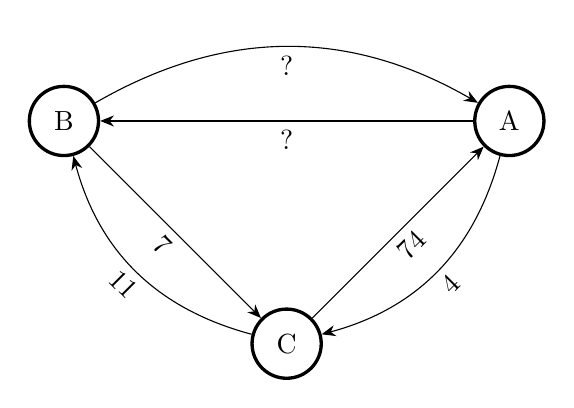
\begin{tikzpicture}[
		node distance = 4cm,
		on grid,
		> = {Stealth[length=5pt,width=4pt]},
		every state/.style = {very thick},
		every edge quotes/.style = {sloped, anchor=north}
		]
		\node[state] (B) {B};
		\node[state] (C) [below right=of B] {C};
		\node[state] (A) [above right=of C] {A};
		\path[->]   
		(A) edge["?"]   (B)
		(B) edge["7"]   (C)
		(C) edge["74"]  (A)
		(B) edge[bend left,"?"]   (A)
		(A) edge[bend left,"4"]   (C)
		(C) edge[bend left,"11"]  (B);
		\end{tikzpicture}
		\caption{Message volume prediction in a social network of 3 users.}
		\label{fig:example}
	\end{figure}
\end{frame}

\begin{frame}{Deep learning approach: Model R (R as in "relation")}
	\begin{figure}[H]
		\centering
		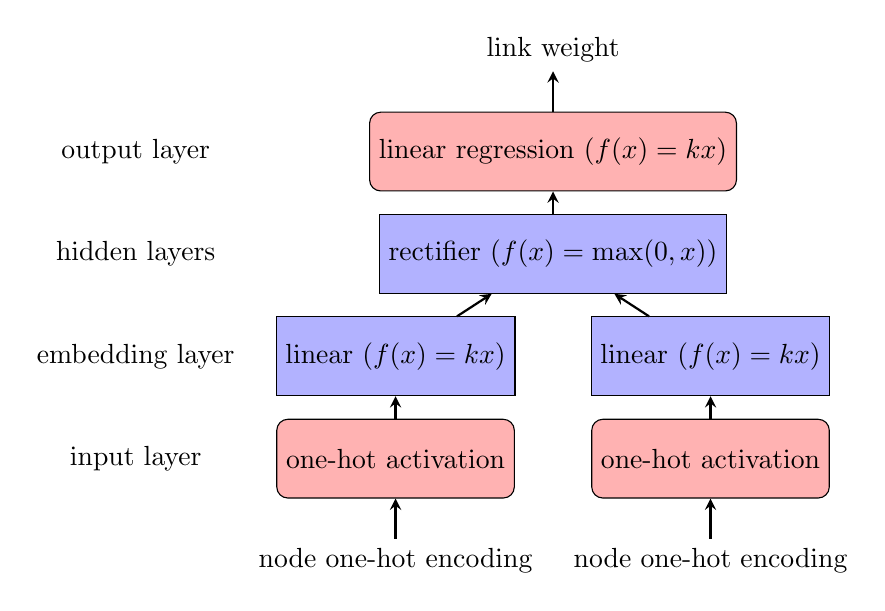
\begin{tikzpicture}[node distance=1.3cm]
		\tikzstyle{startstop} = [rectangle, rounded corners, minimum width=1cm, 
		minimum height=1cm, text centered, draw=black, fill=red!30]
		\tikzstyle{process} = [rectangle, minimum width=1cm, minimum height=1cm, 
		text centered, draw=black, fill=blue!30]
		\tikzstyle{arrow} = [thick,->,>=stealth]
		\node (linearRegression) [startstop] {linear regression ($ f(x) = kx $)};
		\node (relu) [process, below of=linearRegression] {rectifier ($ f(x) = \max (0, x) $)};
		\node (linear1) [process, below of=relu, xshift=-2cm] {linear ($ f(x) = kx $)};
		\node (linear2) [process, below of=relu, xshift=2cm] {linear ($ f(x) = kx $)};
		\node (oneHot1) [startstop, below of=linear1] {one-hot activation};
		\node (oneHot2) [startstop, below of=linear2] {one-hot activation};
		\node (weight) [above of=linearRegression] {link weight};
		\node (output) [left of=linearRegression, xshift=-4cm] {output layer};
		\node (hidden) [below of=output] {hidden layers};
		\node (embedding) [below of=hidden] {embedding layer};
		\node (input) [below of=embedding] {input layer};
		\node (source) [below of=oneHot1] {node one-hot encoding};
		\node (destination) [below of=oneHot2] {node one-hot encoding};
		\draw [arrow] (source) -- (oneHot1);
		\draw [arrow] (destination) -- (oneHot2);
		\draw [arrow] (oneHot1) -- (linear1);
		\draw [arrow] (oneHot2) -- (linear2);
		\draw [arrow] (linear1) -- (relu);
		\draw [arrow] (linear2) -- (relu);
		\draw [arrow] (relu) -- (linearRegression);
		\draw [arrow] (linearRegression) -- (weight);
		\end{tikzpicture}
		\caption{
			Model R with multiple hidden layers.
		}
		\label{fig:model}
	\end{figure}
\end{frame}

\begin{frame}{Experiments: link weight prediction accuracy evaluation}
	\begin{figure}[H]\centering
		\includegraphics[width=\textwidth]{link-weight-errors}
		\caption{
			Model R has lower mean squared errors than 4 baseline approaches over 4 datasets consistently.
		}
		\label{fig:errors}
	\end{figure}
\end{frame}

\begin{frame}{Node embedding analysis}{Motivation}
	\begin{itemize}
		\item Why does Model R perform so well?
		\item What knowledge does Model R learn?
	\end{itemize}
\end{frame}

\begin{frame}{Node embedding analysis}{Dataset: MovieLens 100K}
	\begin{itemize}
		\item Well understood domain: movie recommendation
		\item 100,000 ratings from 1000 users on 1700 movies.
		\item Bigraph: users and movies are nodes; ratings are link weights.
	\end{itemize}
	\begin{figure}[H]\centering
		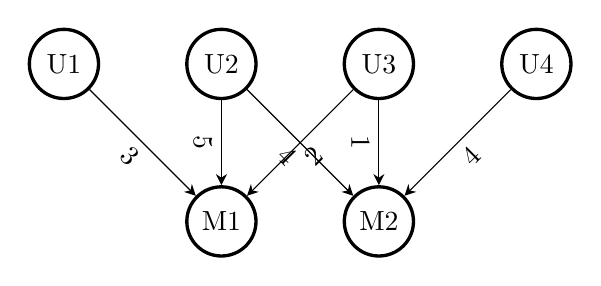
\begin{tikzpicture}[
		node distance = 2cm,
		on grid,
		> = {Stealth[length=4pt,width=4pt]},
		every state/.style = {very thick},
		every edge quotes/.style = {sloped, anchor=north}
		]
		\node[state] (U1) {U1};
		\node[state] (U2) [right =of U1] {U2};
		\node[state] (U3) [right =of U2] {U3};
		\node[state] (U4) [right =of U3] {U4};
		\node[state] (M1) [below=of U2] {M1};
		\node[state] (M2) [right =of M1] {M2};
		\path[->]
		(U1) edge["3"]   (M1)
		(U2) edge["5"]   (M1)
		(U2) edge["4"]  (M2)
		(U3) edge["2"]   (M1)
		(U3) edge["1"]   (M2)
		(U4) edge["4"]   (M2);
		\end{tikzpicture}
		\caption{Movie rating illustration for a dataset of 4 users and 2 movies.}
		\label{fig:movie}
	\end{figure}
\end{frame}

\begin{frame}{Node embedding analysis}{Visualization}
	\begin{figure}[!ht]\centering
		\includegraphics[width=0.6\textwidth]{movies-annotation}
		\caption{
			The embeddings of all movies in MovieLens 100K dataset. Dimensionality reduction of embeddings uses Principal Component Analysis.
		}
		\label{fig:movies}
	\end{figure}
\end{frame}

\begin{frame}{Summary: what Model R can do for us}
	\begin{itemize}
		\item Learn knowledge from past behaviors.
		\item Represent knowledge with numbers.
		\item Use knowledge to predict future behaviors.
	\end{itemize}
	\begin{figure}[H]\centering
		\includegraphics[width=0.7\textwidth]{Social_Network_Analysis_Visualization}
	\end{figure}
\end{frame}
\end{document}